
% \ifltxcounter{letterRot}{}{\newcounter{letterRot}}
% \setcounter{letterRot}{0}

% \newsavebox\letterRotating
% \savebox\letterRotating{
%     \def\do#1{%
%         (#1)%
%     }
%     \docsvlist{A,B,C,D,E,F,G,H}

%     % \begin{tikzpicture}
        
%     % \end{tikzpicture}
% }

\def\pasteframeselection#1{\begin{frame}<#1>}%
    \expandafter\pasteframeselection\expandafter{\frameselection}%
    \frametitle{Code vs Visueel}

    \begin{columns}
        \begin{column}{0.35\textwidth}
            \begin{itemize}
                \item \textbf{Complex}\par
                Formules
                \item<4-> \textbf{Consistent}\par
                Professioneel
                \item<6-> \textbf{Uitbreidbaar}\par
                Packages
            \end{itemize}
        \end{column}
        \begin{column}{0.65\textwidth}
            \only<2>{
                \hll|\\alpha, \\int_0^\{\\infty\}\\sin(x)\\dif x|

                \medskip
                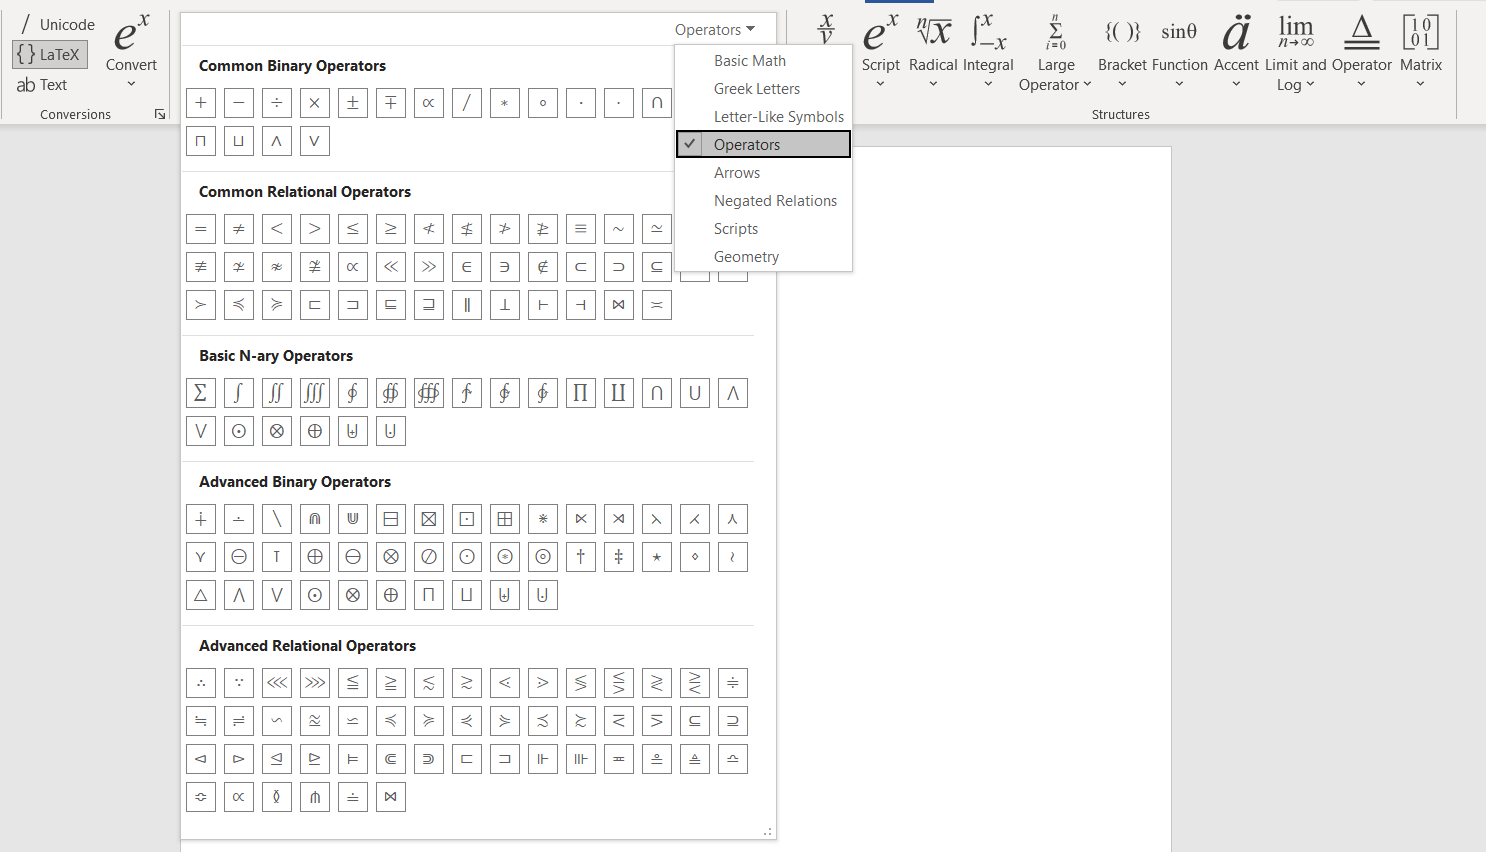
\includegraphics[width=0.9\textwidth]{assets/wordEquationEditorTall.png}
            }
            \only<3>{
                \adjustbox{
                    trim=0pt {0.5\height} {0.5\width} 0pt,clip,width=\linewidth
                }{
                    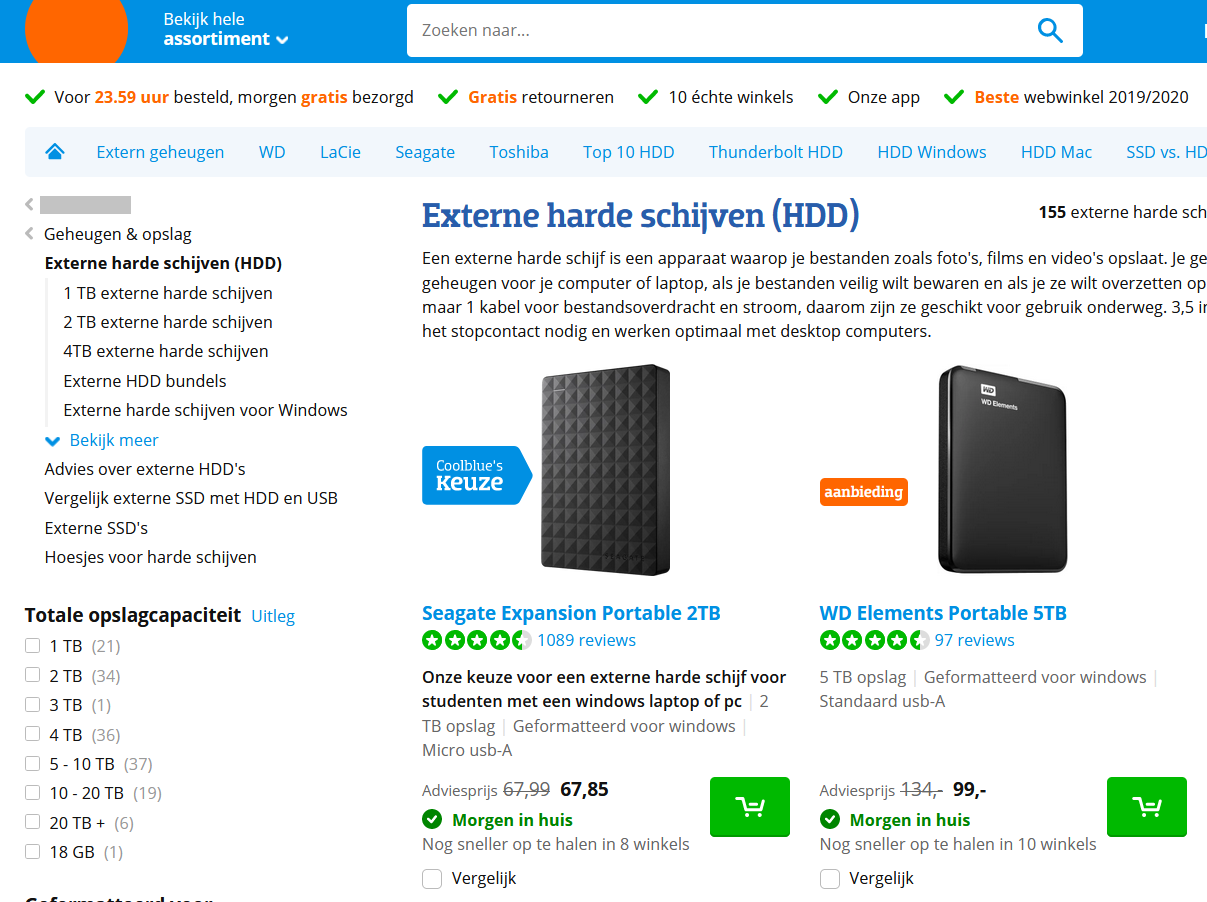
\includegraphics[
                        width=\linewidth,height=0.8\textheight,keepaspectratio
                    ]{assets/websiteVisual.png}
                }
            }
            \only<5>{
                \centering
                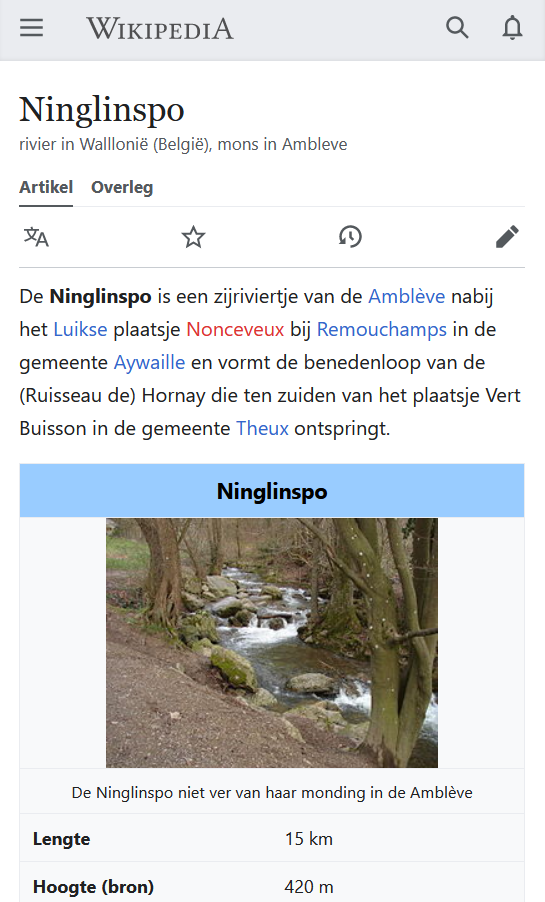
\includegraphics[width=\linewidth,height=0.8\textheight,keepaspectratio]{assets/wikipediaVisual}
            }
            \only<7>{
                %{\setul{1pt}{1pt}\setulcolor{green}\ul{Fanciness}} {\setul{0pt}{1pt}\st{Fancyness}}

                {\setul{1pt}{1pt}\setulcolor{green}\ul{\"F\textsl{\H{a}nc}\^{\i}\~ne\c{s}s}} {\setul{0pt}{1pt}\st{Fancyness}}

                % \textfrak{\so{S{ch}u{tz}vorri{ch}tung}}
                
                % \usebox\letterRotating

                % Maar: \"F\textsl{\H{a}nc}\^{\i}\~ne\c{s}s is vaak DIY, en kost al snel veel moeite!

                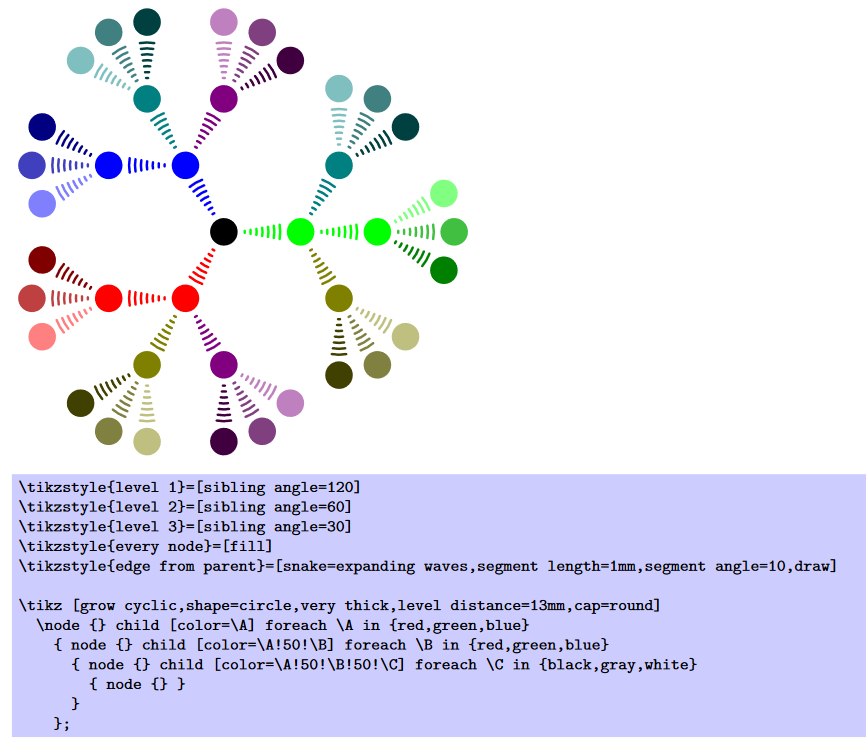
\includegraphics[width=\linewidth,height=0.7\textheight,keepaspectratio]{assets/tikz-showcase.png}
            }
            \only<8>{
                
\includegraphics[width=\linewidth]{assets/whatsappStyles2.png}
        
                \bigskip
                
                %
\includegraphics[width=\linewidth]{whatsappStylesResultCropped.jpg}
                
\includegraphics[width=\linewidth]{assets/whatsappStylesResult2.png}
            }
        \end{column}
    \end{columns}
\end{frame}

\let\frameselection\somethingundefined
